\documentclass[11pt]{article}
\usepackage[margin=1in]{geometry}
\usepackage{amsmath,amssymb,booktabs,hyperref,xcolor,graphicx,multirow}
\usepackage[ruled,vlined]{algorithm2e}
\newcommand{\R}{\mathbb{R}}
\newcommand{\todo}[1]{\textcolor{red}{[#1]}}
\newcommand{\ndcg}{\mathrm{NDCG@}10}
\newcommand{\uk}{u^\star}
\title{\textbf{Just Ask: Open-Vocabulary Free-Recall Preference Elicitation\\Beats Latent Rating-Probes in Cold Start}\\[4pt]
\large Paper D --- working draft}
\author{}
\date{June 2026}
\begin{document}
\maketitle

\begin{abstract}
\noindent Papers~B and~C learned cold-start elicitation \emph{policies} that probe the user with a presented stimulus
(a catalogued concept, or an off-manifold continuous direction $q\in\R^{64}$) and read back a single scalar rating.
Paper~C's continuous policy beat the discrete state of the art on the long tail, but its accuracy edge is marginal and
lives \emph{off-manifold}: the question is a $64$-dimensional vector, not something a person can answer. This paper asks
a simpler question: instead of \emph{guessing} a direction and reading one scalar, why not \emph{ask the user to name}
something they love? An open free-recall question (``name a movie you love'', ``name an underrated film you love'')
returns a \emph{named entity}, which the frozen recommender maps to a full $64$-dimensional item factor---a far
higher-bandwidth answer than a scalar. We show, on the identical recommender, ruler, and budget as Paper~C, that
heuristic open-recall \emph{beats} the learned continuous policy: a popularity-biased answerer (an availability-heuristic proxy) reaches
$\ndcg=0.387$ full ($>$ Paper~C's $0.378$) in $8$ questions, and a \emph{distinctiveness-framed} question (``an
underrated film you love'') reaches $0.382/0.193$ full/tail in only \emph{two} questions---beating Paper~C's
eight-question policy on \emph{both} axes. We further show the \emph{wording} of the open question is a controllable
lever over the head/tail trade-off: ``favourite'' recalls popular (head) titles, ``hidden gem'' recalls distinctive
(tail) titles. We build a \emph{portfolio} of grounded open questions spanning an openness--precision ladder---favourite/hidden-gem/
disliked \emph{movie}, favourite \emph{actor}/\emph{director} (grounded via TMDB credits for the full catalogue), and
favourite \emph{genre}---and show NDCG falls monotonically with grounding coarseness (movie $>$ director $\approx$ D1
$>$ actor $>$ genre) while answerability rises. We then make the asker \emph{deployable}: under a no-repeat
constraint (each distinct question asked once), a REINFORCE-trained policy trained for \emph{every} budget at once acts
as a \emph{questionnaire-design} algorithm---its learned question \emph{sequence} beats the best hand-designed order on
the early-conversation curve (seed-avg $+0.014$ tail at five turns, robust across training seeds), yielding an
\emph{interpretable question sequence}. A modal-path control shows the per-user \emph{branching} it also performs is
value-neutral ($+0.002$ tail; $49$--$63\%$ of users leave the modal path by five turns but the ranking does not move),
so, because the recommender is a permutation-invariant set encoder, the gain is better \emph{sequencing} and adaptivity
buys \emph{efficiency, not a higher ceiling}. A \emph{jointly
trained} open$+$closed policy then learns---on its own---the open-anchor$\to$closed-refine schedule (the closed continuous
probe is unused early and dominates the final turns), the complementarity a frozen bolt-on cannot realise. Against
probe-family baselines on the identical ruler and matched geometric answerer (ConTS, a geometric reduction of PEBOL,
Paper~C's latent probe, entropy-over-concepts), open recall wins on both axes. We close with honest ablations
(REINFORCE beats a differentiable Gumbel trainer for this discrete action; sequencing only helps under the deployability
constraint). LLM realisation and a deployed interface are deferred to the final paper.
\end{abstract}

\section{Introduction \& positioning}
\label{sec:intro}
Cold-start conversational recommenders must build a useful preference belief from a handful of turns. The dominant
paradigm---and the one we developed in Papers~B and~C---is \emph{rating elicitation}: the system \emph{presents} a
stimulus (an item, an attribute/genome concept, or, in Paper~C, a learned continuous direction in the recommender's
latent space) and the user returns a \emph{scalar} judgement (like/dislike, or a graded $[-1,1]$ rating). The policy's
job is to choose the most informative stimulus to present next.

Paper~C pushed this to its logical extreme: a continuous policy that emits an \emph{off-manifold} query
$q\in\R^{64}$---a point \emph{between} the catalogued concepts (mean cosine $0.58$/$0.73$ to the nearest named
concept)---and beat the discrete state of the art on the Cremonesi long tail~\cite{cremonesi10}. But two facts temper that win.
(i)~The accuracy edge is \emph{marginal} on the full metric ($+0.000\text{--}0.006$) and concentrated in the tail
($+0.010$). (ii)~The winning question is \emph{a vector}: no human can answer ``rate the direction
$[0.11,-0.07,\dots]$''. Paper~C's value is real but its mechanism is low-bandwidth (one scalar per turn) and
non-conversational.

\paragraph{The idea.} Turn the protocol around. Rather than the \emph{system} guessing a latent direction and the user
\emph{scoring} it, let the \emph{system} ask an open question and the \emph{user} name an entity:
\emph{``name a movie you love.''} The answer is not a scalar---it is a named item, which the frozen recommender already
embeds as a full $64$-dimensional factor $Q_j$. One open question therefore carries (up to) $64$ dimensions of
preference signal, versus the one dimension a rating-probe recovers. Cold start is exactly the regime where this
matters: the user has salient, extreme favourites they can name instantly, while the rating menu forces them through a
sequence of system-chosen probes.

\paragraph{Contributions.}
\begin{enumerate}
  \item \textbf{Open-recall beats latent rating-probes (\S\ref{sec:headline}).} On the \emph{identical} frozen
  recommender, ruler (ML-1M, te$[300{:}]$, $\ndcg$ full + Cremonesi tail, seed-avg, $8$-question budget) and answer
  grounding as Paper~C, heuristic open free-recall reaches $0.387/0.170$ (availability-proxy answerer; the assumption-free \texttt{random5} gives $0.390/0.185$) and $0.410/0.209$
  (info-favourable answerer) full/tail, versus Paper~C's $0.378/0.178$. No learned asker is required to beat our own
  learned policy.
  \item \textbf{Efficiency (\S\ref{sec:efficiency}).} A single distinctiveness-framed open question already reaches the
  tail level of Paper~C's eight-question policy; \emph{two} such questions ($0.382/0.193$) beat it on \emph{both} axes.
  Open-recall is roughly $4\times$ more sample-efficient.
  \item \textbf{Question-framing as a head/tail lever (\S\ref{sec:framing}).} The \emph{wording} of the open question
  controls what the user recalls and hence where on the popularity spectrum the signal lands: ``favourite'' $\to$
  popular (head), ``underrated/hidden-gem favourite'' $\to$ distinctive (tail). The same protocol spans the head/tail
  trade-off by changing one English phrase.
  \item \textbf{A grounded open-question portfolio and openness--precision ladder (\S\ref{sec:portfolio}).} Item, metadata
  (actor/director, via TMDB credits for the full catalogue), genre, and fully-open ``what do you like?'' questions; NDCG
  falls monotonically with grounding coarseness while answerability rises.
  \item \textbf{A deployable learned asker that designs a better questionnaire (\S\ref{sec:learned}).} Under a no-repeat
  constraint, a belief-conditioned policy trained for \emph{every} budget at once learns a question \emph{sequence} that
  beats the best hand-designed order on the early curve ($+0.014$ tail at five turns, robust over training seeds) and
  yields an \emph{interpretable question sequence}; a modal-path control isolates its per-user \emph{branching} and finds
  it value-neutral ($+0.002$ tail, with $49$--$63\%$ of users off the modal path by five turns), so the win is better
  \emph{sequencing}, not user-conditional routing---permutation invariance means it buys efficiency, not a higher ceiling.
  \item \textbf{A jointly-trained open$+$closed policy (\S\ref{sec:openclosed}).} It learns the open-anchor$\to$
  closed-refine schedule unaided (closed probe unused early, dominant late)---the complementarity a frozen bolt-on
  cannot realise.
  \item \textbf{Baselines and ablations (\S\ref{sec:baselines}--\ref{sec:ablations}).} Probe-family elicitors
  (ConTS~\cite{li21conts}, a geometric reduction of PEBOL~\cite{pebol}, entropy-over-concepts, Paper~C's latent probe) on the identical ruler and matched
  geometric answerer all land below open recall; REINFORCE beats a differentiable Gumbel trainer for this discrete
  action; an honest answerer band (\S\ref{sec:answerer}).
\end{enumerate}

\paragraph{What this paper is \emph{not} (yet).} The user simulator is geometric, not a human or an LLM; we report an
answerer band rather than logged recall (\S\ref{sec:answerer}). The LLM realisation that renders each open question as
free-text and parses free-text answers, and a deployed conversational interface, are the subject of the final paper
(\S\ref{sec:future}). The probe baselines are matched to our geometric answerer, and PEBOL is reproduced as a stated
geometric reduction of its acquisition mechanics, not its original LLM language layer (\S\ref{sec:baselines}).

\section{Setup (shared with Papers~B/C)}
\label{sec:setup}
We reuse Paper~C's experimental apparatus \emph{exactly}, so that any difference is attributable to the elicitation
mechanism and not the measuring stick.

\paragraph{Recommender and ruler.} A frozen V1 set-encoder recommender scores items as $s = b_{\text{pop}} + Q\,u$,
where $u\in\R^{64}$ is the elicited preference belief, $Q\in\R^{|\mathcal I|\times 64}$ the item factors, and
$b_{\text{pop}}$ a popularity bias. We evaluate on MovieLens-1M~\cite{harper15}, test split te$[300{:}]$ ($304$ held-out users),
reporting $\ndcg$ over the full catalogue and over the Cremonesi long tail~\cite{cremonesi10} (head $33\%$ by popularity masked). All
numbers are averaged over seeds $\{1,2,3,7,11\}$ unless noted (exploratory sweeps use $\{1,2,3\}$).

\paragraph{Cold-start protocol.} Each user's rated items are split in half: a \emph{known half} is available to the
elicitation process, and the disjoint \emph{held half} is the ranking target (never folded into $u$). The belief is
$u^\star = \mathrm{enc}(\text{known half})$; the half-fold oracle---folding the entire known half---ceilings the metric
at $\approx 0.41/0.21$ (full/tail). Budget is $8$ questions/turns.

\paragraph{Grounding (shared).} A named entity is grounded by folding its real recommender token: a named movie $j$
contributes its factor $Q_j$ together with the user's residual $\mathrm{resid}_x[j]$, exactly the tokens the encoder
already consumes. No embedding inversion, no SBERT$\to$factor alignment: the open answer reuses the same
$\mathrm{enc}(\cdot)$ as every other path in Papers~B/C.

\section{Open free-recall elicitation}
\label{sec:method}
\paragraph{Protocol.} At turn $t$ the agent poses an open question of a given \emph{type} (favourite, hidden-gem,
disliked, $\dots$). The user---simulated by a fixed recall heuristic (\S\ref{sec:answerer})---\emph{names} an entity
from their known half; we fold its token $(Q_j,\mathrm{resid}_x[j])$ into $u$ and re-rank. This is strictly within the
same $8$-turn, same-encoder budget as Paper~C; the only change is that the \emph{answer} is a named entity (a vector)
rather than a scalar rating of a system-chosen stimulus.

\paragraph{Why higher bandwidth.} A rating-probe turn returns $\mathrm{sign}/\mathrm{cos}(u^\star,q)\in\R^1$. A
free-recall turn returns a named $Q_j\in\R^{64}$. In cold start, where $u^\star$ itself is being assembled from few
observations, the per-turn information of a named item dominates that of a scalar probe---this is the mechanism behind
every result below.

\paragraph{The answerer (simulator).} Because we lack real free-recall logs, the user's choice of \emph{which} item to
name is a heuristic over their known-half rated items. We treat this as the load-bearing assumption and ablate it
across six models (\S\ref{sec:answerer}); crucially we never NDCG-optimise the answerer, which would let the simulated
user name exactly the items that help the recommender (the collusion failure mode proven in Paper~C's answer-learning
ablation). Realistic recall is a popularity-biased sample over the user's $\ge 4$-star items.

\section{Headline: open-recall beats the learned continuous policy}
\label{sec:headline}
Table~\ref{tab:headline} reports $8$-question $\ndcg$ for ``name a movie you love'' under each recall heuristic,
against Paper~C's continuous policy (D1) on the identical ruler.

\begin{table}[t]
\centering
\caption{Open free-recall (``name a movie you love'' $\times 8$) vs.\ Paper~C's learned continuous policy.
ML-1M, te$[300{:}]$, $\ndcg$ full / Cremonesi tail, seed-avg $\{1,2,3\}$. Half-fold ceiling $\approx 0.41/0.21$.}
\label{tab:headline}
\begin{tabular}{llcc}
\toprule
Method & answerer / framing & full & tail \\
\midrule
Paper~C (D1, continuous off-manifold policy) & rating-probe $\times 8$ & 0.378 & 0.178 \\
\midrule
\multirow{6}{*}{Open-recall ``favourite movie'' $\times 8$}
 & \texttt{rating} (info-favourable)        & 0.411 & 0.209 \\
 & \texttt{align} (most-aligned)            & 0.410 & 0.209 \\
 & \texttt{distinct} (hidden-gem framing)   & 0.405 & \textbf{0.211} \\
 & \texttt{random5} (random 5-star; assumption-free) & 0.390 & 0.185 \\
 & \texttt{popweight} (availability proxy; unvalidated) & 0.387 & 0.170 \\
 & \texttt{poppop} (most-famous; pessimistic)& 0.376 & 0.142 \\
\bottomrule
\end{tabular}
\end{table}

\paragraph{Reading the table.} The cleanest, most assumption-free positive is \texttt{random5}---a uniformly random
liked item, no popularity model at all---which beats Paper~C on \emph{both} axes ($0.390/0.185$ vs $0.378/0.178$).
The popularity-biased answerer (\texttt{popweight}, an \emph{availability-heuristic}~\cite{tversky73} \emph{proxy}, not a validated model of
human recall) still beats Paper~C on the full metric ($0.387 > 0.378$) but \emph{loses} the tail ($0.170$ vs
$0.178$): the tail comparison is band-conditional. The info-favourable
answerers reach $0.410/0.209$---essentially the half-fold ceiling---confirming that the \emph{mechanism} (folding named
item factors) has headroom up to the encoder's representational limit. Only the deliberately pessimistic
\texttt{poppop} (the user always names their most famous like) underperforms, and only on the tail, which is exactly
the salience$\leftrightarrow$information tension we make precise in \S\ref{sec:framing}. The take-away: \emph{a fixed
heuristic open-recall schedule beats our own learned continuous policy}, with no asker training.

\section{Efficiency: two open questions beat eight rating-probes}
\label{sec:efficiency}
Table~\ref{tab:kcurve} sweeps the number of open questions $K$. The point is sample efficiency: how few open questions
match Paper~C's eight-turn policy?

\begin{table}[t]
\centering
\caption{Open-recall $K$-sweep. $\ndcg$ full / tail, seed-avg $\{1,2,3\}$. \texttt{distinct}=hidden-gem framing,
\texttt{popweight}=availability proxy. Bold = beats Paper~C D1 ($0.378/0.178$) on that axis.}
\label{tab:kcurve}
\begin{tabular}{lcccc}
\toprule
 & $K{=}1$ & $K{=}2$ & $K{=}4$ & $K{=}8$ \\
\midrule
\texttt{popweight} (availability proxy) full & 0.316 & 0.336 & 0.364 & \textbf{0.387} \\
\texttt{popweight} tail             & 0.112 & 0.133 & 0.152 & 0.170 \\
\texttt{distinct} (hidden-gem) full & 0.355 & \textbf{0.382} & \textbf{0.396} & \textbf{0.405} \\
\texttt{distinct} tail              & \textbf{0.174} & \textbf{0.193} & \textbf{0.202} & \textbf{0.211} \\
\bottomrule
\end{tabular}
\end{table}

\paragraph{Two questions, both axes.} A single hidden-gem question ($K{=}1$, \texttt{distinct}) already matches
Paper~C's \emph{tail} ($0.174$ vs.\ $0.178$). \emph{Two} hidden-gem questions ($0.382/0.193$) beat Paper~C's
eight-turn policy on \emph{both} the full and tail metrics. Open-recall is therefore $\approx 4\times$ more
sample-efficient than rating-probing in this regime---each named item is worth roughly four direction-probes, the
quantitative signature of the bandwidth argument.

\section{Question framing is a head/tail lever}
\label{sec:framing}
The recall heuristic is a proxy for the \emph{wording} of the open question, and Table~\ref{tab:kcurve} shows the
wording controls where the elicited signal lands on the popularity spectrum. Figure~\ref{fig:framing_lever} confirms
the lever directly on an LLM-simulated user: swapping one word shifts the named title $-33$ percentile points toward
the tail.

\begin{itemize}
  \item \textbf{``Name a favourite movie''} $\to$ users recall \emph{popular} titles (\texttt{popweight}/\texttt{poppop}).
  Strong on the full metric (head items dominate it) but weak on the tail---a famous favourite says little about niche
  taste.
  \item \textbf{``Name an underrated film you love''} $\to$ users recall \emph{distinctive, low-popularity} titles
  (\texttt{distinct}). Far stronger on the tail ($0.193$ vs.\ $0.133$ at $K{=}2$) because a niche favourite is
  diagnostic of exactly the long-tail preferences the head-popularity prior cannot supply.
\end{itemize}

\begin{figure}[t]
\centering
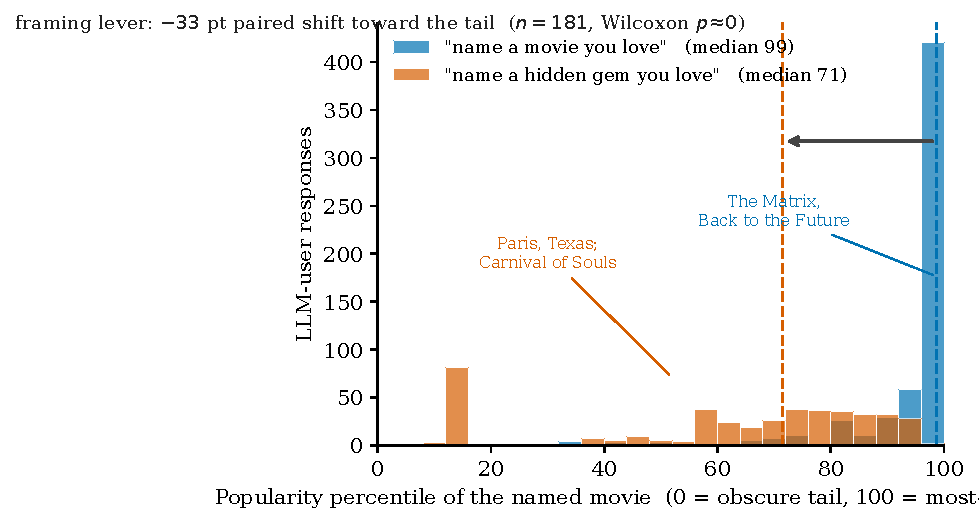
\includegraphics[width=0.92\linewidth]{figs/fig_framing_lever.pdf}
\caption{\textbf{The framing lever, measured on an LLM-simulated user.} Popularity percentile of the movie a
\texttt{gpt-4o-mini} user names when asked, in identical context, ``name a movie you love'' (blue) vs.\ ``name a
hidden gem you love'' (orange). One English word moves the recalled title a \textbf{paired $-33$ percentile points
toward the long tail} ($n{=}181$ users, Wilcoxon $p\!\approx\!0$; medians $99\!\to\!71$): ``love'' recalls the head
(\emph{The Matrix}, \emph{Back to the Future}); ``hidden gem'' recalls the tail (\emph{Paris, Texas}, \emph{Carnival of
Souls}). The lever the model assumes is real in a stand-in user, and it is a single-phrase design knob---exactly the
head/tail control this section claims.}
\label{fig:framing_lever}
\end{figure}

This is a genuinely useful and, to our knowledge, novel control surface: the same open-recall protocol spans the
head/tail trade-off by changing a single English phrase, with no change to the model or budget. It also predicts the
right design for a \emph{learned} asker---one that chooses ``favourite'' when it needs to nail the head and ``hidden
gem'' when it needs to resolve the tail (\S\ref{sec:future}).

\section{An open-question portfolio: items first, then up to ``what do you like?''}
\label{sec:portfolio}
``Favourite movie'' is the first and most precise open question, but a single type cannot span a user's preference
geometry. We build a \emph{portfolio} of item-grounded open questions, each grounded by the same token-fold
(\S\ref{sec:setup}), spanning positive/negative and head/tail recall:
\begin{description}
  \item[\texttt{fav}] highest-rated favourite---a \emph{head} anchor, precise and high-confidence.
  \item[\texttt{gem}] underrated/hidden-gem favourite (high alignment, low popularity)---\emph{tail}-discriminating.
  \item[\texttt{hate}] a movie you disliked---a \emph{negative} token that prunes the wrong region of taste space.
\end{description}

\begin{table}[t]
\centering
\caption{Item-grounded open-question \emph{portfolio} ($8$ questions split across types), vs.\ Paper~C. $\ndcg$
full / tail, seed-avg $\{1,2,3\}$. Here \texttt{fav}/\texttt{gem} use the info-favourable (highest-rated /
high-align-low-pop) recall, so these are the upper band; the availability-proxy operating point follows Table~\ref{tab:headline}.
Bold = best on that axis.}
\label{tab:portfolio}
\begin{tabular}{lcc}
\toprule
portfolio (8 questions) & full & tail \\
\midrule
Paper~C (D1)                       & 0.378 & 0.178 \\
\texttt{fav}:8 (all favourite)     & \textbf{0.411} & 0.209 \\
\texttt{gem}:8 (all hidden-gem)    & 0.405 & 0.211 \\
\texttt{fav}:4 \texttt{gem}:4      & 0.409 & \textbf{0.211} \\
\texttt{fav}:3 \texttt{gem}:3 \texttt{hate}:2 & 0.406 & 0.209 \\
\texttt{fav}:2 \texttt{gem}:4 \texttt{hate}:2 & 0.404 & 0.211 \\
\texttt{gem}:6 \texttt{hate}:2     & 0.400 & 0.210 \\
\bottomrule
\end{tabular}
\end{table}

\paragraph{What the portfolio buys.} All-favourite ($0.411$) maximises the full metric (head titles dominate it);
mixing in hidden-gem questions (\texttt{fav}:4 \texttt{gem}:4, $0.409/0.211$) trades a hair of full for the best tail,
realising in one schedule the head/tail lever of \S\ref{sec:framing}. Adding \emph{disliked}-movie (\texttt{hate})
tokens does \emph{not} help on this ruler---a negative item prunes less than a positive item informs when the budget is
scarce---so the productive item portfolio is positive-recall (favourite~$+$~hidden-gem), with the mix governing the
head/tail balance. These numbers use info-favourable recall (upper band); the availability-proxy portfolio sits
proportionally lower, tracking Table~\ref{tab:headline}.

\paragraph{Roadmap: items $\to$ metadata $\to$ themes $\to$ open.} The portfolio generalises along a ladder of
increasing openness and decreasing groundedness:
\begin{enumerate}
  \item \textbf{Items} (\S\ref{sec:portfolio}): favourite / hidden-gem / disliked movie $\to$ item factor. Most precise,
  no extra metadata.
  \item \textbf{Metadata} (\S\ref{sec:metadata}): favourite \emph{actor} / \emph{director} $\to$ centroid of their
  films' factors. Objective, easy for users to answer; uses TMDB cast/crew.
  \item \textbf{Themes/mood} (\S\ref{sec:metadata}): favourite \emph{genre} $\to$ genre centroid (and, in future,
  ``what do you watch to relax'' $\to$ genome/mood concept). Coarser, broader coverage, more subjective.
  \item \textbf{Fully open} (future): ``what do you like?'' $\to$ free text grounded to the nearest entity/concept.
  Highest openness, lowest precision; the deployable end-state and the natural bridge to LLM realisation.
\end{enumerate}
Objective recall (movie/actor/director) is known to be more reliable for users than subjective recall (mood); we weight
the portfolio toward the grounded, objective end and treat fully open questions as the deployability frontier.
Sections~\ref{sec:metadata} measures rungs 1--3; rung 4 is future work.

\subsection{Beyond items: metadata-grounded open questions}
\label{sec:metadata}
The next rung is \emph{metadata} recall: ``name a favourite actor / director.'' Such questions are attractive because
they are \emph{objective} (a user names a person more reliably than they rate a latent direction) and \emph{broad-
coverage} (one name implicates an entire filmography), but they are \emph{coarser} than item recall: a named person
grounds not to a single item factor but to the \emph{centroid of that person's catalogue films}---which is all the
system can infer from the name alone, independent of which of their films the user actually saw. We obtain top-billed
cast and directors for the full ML-1M catalogue from TMDB (via the MovieLens \texttt{links} mapping), map each person to
the centroid of their films' factors, and have the simulated user name the most salient favourite person from their
known-half liked films (by film-count, by rating, or by centroid alignment), folding the person-centroid token.

We obtain credits for $3{,}666$ of the $3{,}706$ ML-1M titles ($8{,}569$ distinct actors, $1{,}972$ directors).
Table~\ref{tab:metadata} reports metadata recall, the coarsest genre rung, and the open$+$closed mix.

\begin{table}[t]
\centering
\caption{Metadata- and theme-grounded open recall ($8$ names unless noted), and the open$+$closed mix. $\ndcg$ full /
tail, seed-avg $\{1,2,3\}$. \texttt{count}$=$most-named person (realistic salience); \texttt{align}$=$most-characteristic
person (info-favourable); a person/genre grounds to its films' centroid.}
\label{tab:metadata}
\begin{tabular}{lcc}
\toprule
open question & full & tail \\
\midrule
favourite \emph{movie} (item, \texttt{align}) & \textbf{0.410} & \textbf{0.209} \\
Paper~C (D1, continuous rating-probe) & 0.378 & 0.178 \\
\midrule
favourite \emph{actor} (\texttt{count}, realistic)   & 0.369 & 0.154 \\
favourite \emph{actor} (\texttt{rating})             & 0.377 & 0.160 \\
favourite \emph{actor} (\texttt{align}, info-fav.)   & 0.408 & 0.203 \\
favourite \emph{director} (\texttt{count})           & 0.378 & 0.180 \\
favourite actor $+$ director (\texttt{both}, \texttt{count}) & 0.379 & 0.166 \\
\midrule
favourite \emph{genre} ($\times 3$, \texttt{count})  & 0.346 & 0.108 \\
favourite \emph{genre} ($\times 3$, \texttt{align})  & 0.340 & 0.143 \\
\midrule
mix: 4 actors $+$ 4 favourite movies (\texttt{count}) & 0.409 & 0.203 \\
\midrule
fully-open ``what do you like?'' (union, info-fav.) & 0.407 & 0.206 \\
fully-open, availability proxy ($\equiv$ \texttt{popweight} movie) & 0.387 & 0.170 \\
\bottomrule
\end{tabular}
\end{table}

\paragraph{The openness--precision ladder.} The results trace a clean ladder. Under \emph{realistic} recall, NDCG falls
monotonically with the coarseness of the grounding: favourite movie ($0.39$, Table~\ref{tab:headline}) $>$ director
($0.378$) $\approx$ D1 $>$ actor ($0.369$) $>$ genre ($0.346$). A named person or genre grounds to a \emph{centroid}
that averages a whole filmography, so it is necessarily less precise than a named title---this is the honest cost of
moving up the openness ladder. Three findings sharpen the picture:
\begin{itemize}
  \item \textbf{Directors beat actors, per name.} Even under realistic count-recall, a director-name ($0.378/0.180$)
  out-informs an actor-name ($0.369/0.154$) on \emph{both} axes, and matches D1. A director's filmography is
  stylistically more coherent (an auteur signal) than an actor's, so its centroid is a tighter preference token.
  \item \textbf{The ceiling is high when the \emph{right} person is named.} The info-favourable
  \texttt{align} actor ($0.408/0.203$) nearly matches favourite-movie recall: a well-chosen actor centroid is almost as
  informative as a named title. The realistic--optimistic band ($0.369$--$0.408$) is the metadata analogue of
  Table~\ref{tab:headline}'s answerer band.
  \item \textbf{Fewer, coarser names is better.} For genres, naming $3$ beats naming $8$ (Table omits $K{=}8$:
  $0.327/0.101$): piling on coarse tokens drags the belief toward a generic centroid. Coarse questions saturate fast.
\end{itemize}

\paragraph{Open $+$ closed mix.} Metadata's real value is \emph{answerability and coverage}---a person is objective and
easy to name, and one name implicates many films---not peak NDCG. The natural design therefore \emph{mixes} a cheap
objective opener with precise item anchors: $4$ favourite actors $+$ $4$ favourite movies reaches $0.409/0.203$ under
realistic recall, recovering essentially the full favourite-movie performance while front-loading the conversation with
the easiest-to-answer questions. This is the first concrete instance of the open$+$closed mixing the protocol allows.

\subsection{The fully-open question, and why wording still matters}
\label{sec:fullyopen}
The top of the ladder is the maximally unconstrained question---\emph{``what do you like?''}---where the user may
volunteer \emph{any} entity. We model this as a \emph{union} answer space (every movie, actor, director, and genre
implicated by the user's known-half likes), ranked by alignment to $u^\star$ so the types are comparably scaled; this is
the \emph{info-favourable} fully-open answerer. It reaches $0.407/0.206$---essentially item-level---and, tellingly, when
free to name anything optimally the user names a \emph{person} $68\%$ of the time, a movie $29\%$, a genre $3\%$: a
well-aligned actor centroid implicates many on-target films, so it is the highest-coverage single name. Maximal openness,
\emph{if answered optimally}, costs almost nothing.

\paragraph{But generic openness forfeits the framing lever.} The catch is that a single generic question cannot
\emph{steer} where the signal lands. Realistically, ``what do you like?'' elicits a popular, top-of-mind \emph{movie}---
the \texttt{popweight} favourite ($0.387/0.170$): healthy on the full metric, but its tail ($0.170$) sits well below what
a \emph{targeted} hidden-gem question reaches in just two turns ($0.193$, Table~\ref{tab:kcurve}). The head/tail lever of
\S\ref{sec:framing} \emph{requires} a worded question; the fully-open question trades that control away. This is the
paper's closing point: openness is cheap in the \emph{recall mechanism} but the \emph{value lives in the wording}---a
designed open question (``an underrated film you love'') beats the generic one (``what do you like?'') precisely on the
long tail, which is where cold-start recommendation is hard.

\section{The deployable setting and a learned anytime asker}
\label{sec:learned}
So far the asker has been a \emph{fixed schedule}. Two facts now force a more careful treatment. First,
\emph{deployability}: asking ``name an underrated film you love'' eight times in a row is not a real conversation---a
deployed agent asks each \emph{distinct} question at most once. Second, \emph{structure}: our recommender is a
\emph{permutation-invariant set encoder}, so after a fixed set of answers the belief---and hence the final NDCG---does
\emph{not} depend on the order they were given. Adaptivity therefore cannot raise the full-budget ceiling; its only
lever is the \emph{shape of the curve}: which question to ask \emph{first}, and which to ask next given the answers so
far, to reach good NDCG \emph{sooner}.

\subsection{The no-repeat action space}
We assemble a catalogue of distinct open questions, each grounded as in \S\ref{sec:setup}: ``name a movie you love''
(with the framing lever, \S\ref{sec:framing}, realised as the \texttt{favourite}/\texttt{hidden-gem}/\texttt{all-time}
variants), ``a movie you disliked'', ``a favourite genre'', ``a genre you avoid'', ``a favourite actor'', ``a favourite
director'', and ``what do you like?''. This is $\approx 6$--$7$ \emph{semantically distinct} questions (the three
movie-framings share a question and differ only in wording), $\approx 8$--$9$ grounding types in all. Under the
\emph{no-repeat} constraint each type is asked at most once, so the open budget is bounded by the catalogue size---a
concrete answer to ``how many open questions do we have before going closed?'': about eight.

\subsection{The policy and its objective}
Let $b_t=\mathrm{enc}(\{(\phi_s,a_s)\}_{s<t})\in\R^{64}$ be the belief after the first $t$ answers (the same encoder the
recommender uses). A policy $\pi_\theta(\cdot\mid b_t,t)$ outputs a distribution over the question types still available
(exhausted and already-asked types are masked). Because the chosen type deterministically fixes which entity the
simulated user recalls (\S\ref{sec:answerer}), the only learned decision is \emph{which type to ask}. Crucially, at
$t{=}0$ the belief is $b_0=\mathrm{enc}(\varnothing)=\mathbf 0$ for \emph{every} user, so a realizable policy must emit
the \emph{same opener} for all users---the per-user adaptivity can only begin at $t\ge 1$, once an answer has
differentiated the belief.

We train for \emph{every} budget at once (an ``anytime'' objective), rewarding the mean ranking quality across all turns
rather than only the last:
\begin{equation}
\label{eq:anytime}
J(\theta)=\mathbb{E}_{\pi_\theta}\!\left[\tfrac{1}{T}\sum_{t=1}^{T}\big(\,w_f\,\ndcg^{\mathrm{full}}_t+w_t\,\ndcg^{\mathrm{tail}}_t\,\big)\right],
\qquad \ndcg_t=\ndcg\big(\,b_t\,\big),
\end{equation}
optimised by REINFORCE with a batch-mean baseline (the action is a discrete categorical, so the score-function
estimator~\cite{williams92} applies directly; we revisit a differentiable alternative in \S\ref{sec:trainer}). Algorithm~\ref{alg:asker}
gives the rollout.

\begin{algorithm}[t]
\caption{Anytime no-repeat open-question asker (one training rollout)}
\label{alg:asker}
\KwIn{user with known half $H$; encoder $\mathrm{enc}$; recommender $s=b_{\mathrm{pop}}+Q\,b$; budget $T$; recall map
$\rho(\text{type},H)\!\to\!(\phi,a)$}
$\mathcal{A}\leftarrow$ available types;\quad $b\leftarrow\mathbf 0$;\quad tokens $\leftarrow[\,]$;\quad $R\leftarrow 0$\;
\For{$t=1$ \KwTo $T$}{
  $p\leftarrow \pi_\theta(\cdot\mid b,t)$ with already-asked / exhausted types masked to $-\infty$\;
  sample type $k\sim p$ (greedy $\arg\max$ at eval); append $\rho(k,H)$ to tokens; mark $k$ used\;
  $b\leftarrow \mathrm{enc}(\text{tokens})$;\quad $R\mathrel{+}= \tfrac1T\big(w_f\,\ndcg^{\mathrm{full}}(b)+w_t\,\ndcg^{\mathrm{tail}}(b)\big)$\;
}
update $\theta$ by REINFORCE on $R$ with a batch-mean baseline\;
\end{algorithm}

\subsection{Fixed vs.\ adaptive: the learned asker improves the early curve}
Table~\ref{tab:curve} reports the per-turn curve of the learned policy against the best fixed order, both belief-only
and realizable (no privileged features; opener fixed across users), seed-averaged over three training seeds and three
evaluation seeds.

\begin{table}[t]
\centering
\caption{Learned anytime asker vs.\ fixed no-repeat order. $\ndcg$ full / tail, te$[300{:}]$, seed-avg. The learned
policy wins on the early/mid curve, especially the tail; the two converge at the full-budget endpoint (permutation-
invariant encoder). Robust across $3$ training seeds.}
\label{tab:curve}
\begin{tabular}{lcccccc}
\toprule
turn & 1 & 2 & 3 & 5 & 6 & 8 \\
\midrule
fixed order (full)   & 0.355 & 0.375 & 0.387 & 0.393 & 0.393 & 0.405 \\
\textbf{learned (full)} & 0.371 & 0.385 & 0.389 & \textbf{0.398} & \textbf{0.398} & 0.405 \\
\midrule
fixed order (tail)   & 0.173 & 0.167 & 0.170 & 0.177 & 0.176 & 0.195 \\
\textbf{learned (tail)} & 0.172 & \textbf{0.188} & \textbf{0.190} & \textbf{0.190} & \textbf{0.190} & 0.194 \\
\bottomrule
\end{tabular}
\end{table}

\begin{figure}[t]
\centering
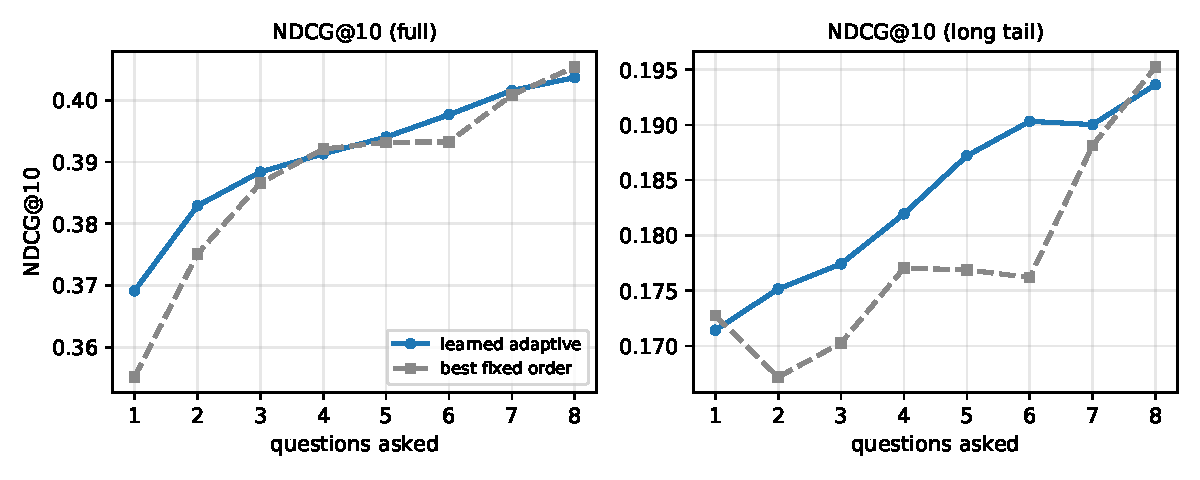
\includegraphics[width=0.92\linewidth]{fig_anytime_curve.pdf}
\caption{Anytime no-repeat curves: the learned anytime asker (solid) vs.\ the best hand-designed order (dashed), full and
long-tail NDCG@10 by number of questions asked. The learned \emph{sequence} reaches good quality earlier---most visibly
on the tail---and converges at the full budget, as the permutation-invariant encoder requires. A modal-path control
(\S\ref{sec:tree}) shows the gain is better sequencing, not per-user branching; adaptivity buys efficiency, not a higher
ceiling.}
\label{fig:curve}
\end{figure}

\textbf{The win is better sequencing, not per-user branching.} REINFORCE acts here as a \emph{questionnaire-design}
algorithm. The learned question \emph{sequence} reaches the hand-designed order's eventual tail quality several turns
earlier (Figure~\ref{fig:curve}, consistently positive over turns $2$--$7$), and converges at $t{=}8$ as the encoder's
permutation invariance requires; a five-seed evaluation puts the $t{=}5$ gap over the hand-designed order at $+0.004$
full / $+0.014$ tail, robust across training seeds. A \emph{modal-path control} then isolates how much of this gain is
genuine \emph{per-user branching} versus simply a better \emph{static} order: freezing each trained policy into its own
single most-frequent question sequence---its \emph{modal path}---and running that as a fixed schedule recovers almost all
of the gain, so branching adds only $+0.001$ full / $+0.002$ tail over the modal-static order ($\approx0$). The policies \emph{do} branch
heavily---$49$--$63\%$ of users leave the modal path by $t{=}5$---but that branching is \emph{value-neutral}: consistent
with a permutation-invariant encoder in a near-linear world, the answers carry no routing signal that a good static
front-loading has not already captured. The honest claim is therefore that \emph{RL discovers a better static
questionnaire with anytime front-loading, not user-conditional routing}; \emph{adaptivity buys efficiency, not a higher
ceiling}---a deployable win precisely where a real session is short.

\subsection{What the policy learned: an interpretable tree}
\label{sec:tree}
Because the action is a named question, the greedy policy is directly readable as a decision tree over question types
(Figure~\ref{fig:tree}). It \emph{opens}, for every user, with a single high-bandwidth recall---``your all-time
favourite''---then \emph{branches on the answer}: the bulk of users ($67\%$) are next asked their favourite \emph{genre},
others their \emph{favourite} or a \emph{favourite actor}; deeper in the tree, once the head of the profile is pinned,
the policy turns to \emph{hidden-gem} and \emph{disliked} questions that resolve the long tail. The opener is fixed
across users (as it must be---at $t{=}0$ every belief is $\mathbf 0$, \S\ref{sec:learned}); the branching from $t\ge 2$
is genuinely belief-conditioned ($49$--$63\%$ of users leave the modal path by $t{=}5$). As the modal-path control above
established, however, that branching is \emph{value-neutral}: freezing this seed's modal question order into a static
schedule recovers almost all of the gain over the hand-designed order (branching residual $+0.001$ full / $+0.002$ tail),
so the tree is best read as \emph{one seed's learned questionnaire order} rather than a routing policy whose branches pay.
It recovers, as a \emph{learned} sequence, exactly the head-then-tail logic the framing lever predicted by hand
(\S\ref{sec:framing}): pin the head with a precise favourite and a coarse genre, then spend later turns on the
distinctive and negative questions that move the tail.

\begin{figure}[t]
\centering
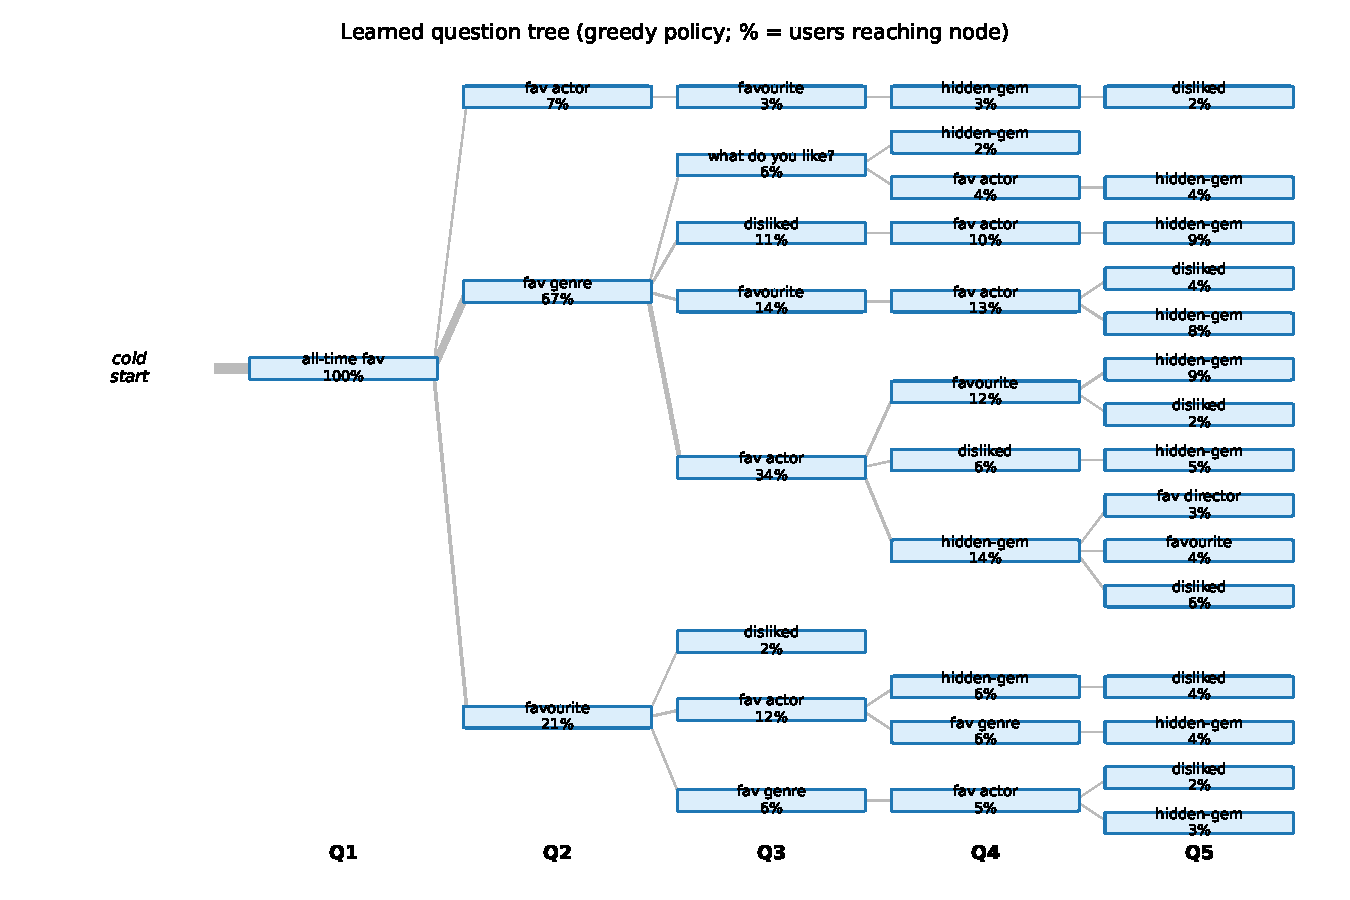
\includegraphics[width=\linewidth]{fig_learned_tree.pdf}
\caption{One training seed's learned question order, drawn as a tree over question types (greedy policy on test users;
\% is the fraction of users reaching each node). The opener is fixed (``all-time favourite''); the policy then branches
on the answer, pinning the head (genre/favourite/actor) before turning to hidden-gem and disliked questions for the tail.
The tree visualises \emph{one seed's learned sequence}; a modal-path control (\S\ref{sec:tree}) shows the per-user
branching it depicts is \emph{value-neutral}---almost all the gain over the hand-designed order comes from the better
static ordering, not the branching. An interpretable, deployable questionnaire learned purely from NDCG.}
\label{fig:tree}
\end{figure}

\section{Open $+$ closed: a jointly-trained policy mixes recall and probing}
\label{sec:openclosed}
The natural endpoint is a policy whose action set is the \emph{union} of the open-recall questions above \emph{and} the
\emph{closed continuous probe of Paper~C}. Concretely, the \texttt{closed} action invokes Paper~C's \emph{trained}
continuous actor: from the current belief it emits an off-manifold latent query $q\in\R^{64}$ and reads back the graded
geometric answer $a=\mathrm{NEG}+(\mathrm{POS}-\mathrm{NEG})\,(\cos(\uk,q){+}1)/2$, exactly as in Paper~C. This is the
same low-bandwidth rating-probe the rest of this paper argues against---included here precisely to test whether a learned
policy finds any residual use for it alongside high-bandwidth recall. The closed probe is \emph{repeatable}---each probe
is a fresh adaptive direction conditioned on the running belief, not a catalogue entry---so it is exempt from the
no-repeat constraint and is not capped by the catalogue size.

\paragraph{Bolt-on fails; joint training succeeds.} A naive bolt-on---$k$ fixed open turns, then the \emph{frozen}
Paper~C probe policy for the remainder---\emph{never} beats pure open recall, and for the availability-proxy answerer dips
\emph{below} both endpoints (e.g.\ $2$ open $+$ $6$ probe $=0.341/0.132$ vs.\ pure-open $0.387/0.170$): the probe is
lower-bandwidth and the Paper~C actor is off-distribution on an open-seeded belief. But a \emph{jointly trained} policy
over the union learns to use the two complementarily. Table~\ref{tab:closedmix} shows it edges the open-only asker on
the tail, and---decisively for interpretability---it learns the \emph{open-anchor $\to$ closed-refine} schedule on its
own: the closed probe is essentially unused early and dominates the final turns.

\begin{table}[t]
\centering
\caption{Closed-probe usage by turn (seed-avg, greedy policy) and NDCG of the jointly-trained open$+$closed asker.
The policy recalls early, then refines with repeatable continuous probes.}
\label{tab:closedmix}
\begin{tabular}{lcccccccc}
\toprule
turn & 1 & 2 & 3 & 4 & 5 & 6 & 7 & 8 \\
\midrule
\% closed-probe & 0 & 0 & 0 & 0 & $\sim$4 & $\sim$18 & $\sim$30 & $\sim$67 \\
\bottomrule
\end{tabular}\\[4pt]
\small open$+$closed (joint): $0.400/0.193$ at $t{=}5$, $0.405/0.197$ at $t{=}8$ \;($\approx{+}0.003$ tail over
open-only; both $\gg$ fixed $0.393/0.177$ at $t{=}5$).
\end{table}

This is the cleanest statement of the combine question: \emph{open recall and closed probing are complementary, but only
a jointly trained policy can exploit it}---the bolt-on is a negative, the joint policy a (modest) positive, and the
learned closed-usage curve makes the mechanism legible.

\section{Baselines: published elicitors on the same ruler}
\label{sec:baselines}
We compare against the probe-family elicitors on the \emph{identical} recommender, answerer, and metric. The
probe baselines all \emph{present} a stimulus the user rates; our methods have the user \emph{recall} an entity.

\paragraph{Matched answerer, no peeking.} Every baseline answers from the \emph{known-half} geometry
$\uk=\mathrm{enc}(H)$ (a concept/aspect $\phi$ yields $a=\uk\!\cdot\hat\phi$); the held target is used only to score
NDCG, never to answer. This is identical to our own answerer and is in fact \emph{stricter} than the original PEBOL,
whose simulator answers from the held target. Crucially, every method runs the \emph{identical} deployable protocol: the asker is \emph{blind} to the profile (it may
ask any concept), an unanswerable question \emph{wastes the turn} (the user, who knows only their own history, refuses),
and the ConTS~\cite{li21conts} arm set / PEBOL~\cite{pebol} per-item Beta range over a \emph{shared, popularity-stratified candidate pool} (identical
across users), not the user's own items. So no acquisition can peek at the very profile it is meant to elicit. (Relaxing
either constraint---pre-filtering to answerable concepts, or grounding the belief on the known-half items---inflates the
probes substantially, e.g.\ PEBOL from $0.317/0.092$ to $0.369/0.168$; we report only the leak-free, blind-refuse
numbers, matched to our own methods.)

\paragraph{Geometric reductions (stated plainly).} \textbf{ConTS}~\cite{li21conts} is reproduced faithfully---a Bayesian-linear
posterior over $u$ with Thompson sampling over a unified arm set of concepts and a shared item pool. \textbf{PEBOL}~\cite{pebol} is
reproduced \emph{as a geometric reduction}: its load-bearing mechanics (a Beta belief per item over the shared pool,
Thompson acquisition over aspects)
are preserved, but its two LLM components---GPT aspect generation and BART-NLI grounding---are replaced by our concept
embeddings and a geometric entailment $w_i=\sigma(\tau\,\hat\phi\!\cdot\!\hat Q_i)$. This is defensible precisely because
our thesis is that the response is geometric, so no language layer is needed; but it is \emph{not} the original LLM
system, and we report it as such. \textbf{GATE}~\cite{gate} and the general$\to$specific funnel~\cite{montazeralghaem25} are off-ruler by construction
(binary-label AUC and BLEU/ROUGE reconstruction respectively, with no recommender); we cite them as related work rather
than fabricate a leaderboard row. \textbf{Sanner et al.\ (2023)}~\cite{sanner23} is a one-shot full-named-profile method, not a
turn-budgeted policy; it is the no-budget reference, not a competitor.

\begin{table}[t]
\centering
\caption{Paper-D comparison, all on the identical ML-1M ruler, known-half geometric answerer, $8$-turn budget,
seed-avg te$[300{:}]$. Probe baselines \emph{present}; our methods \emph{recall}.}
\label{tab:baselines}
\begin{tabular}{llcc}
\toprule
 & method & full & tail \\
\midrule
\multirow{4}{*}{probe (present)}
 & ConTS (Thompson, concept$+$shared-pool arms) & 0.309 & 0.089 \\
 & PEBOL-geometric (Beta $+$ aspect Thompson)  & 0.317 & 0.092 \\
 & entropy-over-concepts (Paper~B)             & 0.361 & 0.140 \\
 & Paper~C D1 (continuous latent probe)       & 0.378 & 0.178 \\
\midrule
\multirow{3}{*}{recall (ours)}
 & fixed open-recall schedule                 & 0.405 & 0.195 \\
 & learned anytime asker                      & 0.405 & 0.194 \\
 & open $+$ closed (joint)                    & \textbf{0.405} & \textbf{0.197} \\
\bottomrule
\end{tabular}
\end{table}

\paragraph{Reading the table.} Every probe elicitor---the literature's BO/bandit methods (PEBOL $0.317/0.092$, ConTS
$0.309/0.089$), our concept-entropy policy ($0.361/0.140$), and our own Paper~C latent probe ($0.378/0.178$)---lands
below open recall on both axes. Even the strongest probe (the Paper~C continuous latent, $0.378/0.178$) sits $0.027$
full / $0.017$ tail under the open asker, and the strongest \emph{literature} probe (PEBOL-geometric) sits $0.088$ full
/ $0.103$ tail under it. The gap reflects the paper's thesis (a probe reads one scalar about a
\emph{system-chosen} stimulus; recall folds a full factor about a \emph{user-volunteered} one), measured under a matched
answerer; we do not claim it refutes the original LLM systems, only that on this ruler the \emph{interaction} of
free-recall dominates probing.

\section{Ablations}
\label{sec:ablations}
\paragraph{Trainer: REINFORCE vs.\ differentiable Gumbel (\S\ref{sec:trainer}).}
\label{sec:trainer}
Paper~C trained a \emph{continuous} action by back-propagating a differentiable soft-NDCG. Paper~D's action is a
\emph{discrete} categorical, so we default to REINFORCE~\cite{williams92} on the exact reward; we also implemented the differentiable
alternative---Gumbel-softmax~\cite{jang17gumbel} straight-through over the type choice, with Paper~C's soft-NDCG through a torch encoder
fold. The differentiable variant \emph{underperforms} ($0.400/0.185$ vs.\ REINFORCE $0.405/0.194$ at $t{=}8$, worse on
the tail), because the soft-NDCG surrogate ranks held-likes against \emph{popular} negatives---a full-metric objective
misaligned with the exact tail-weighted $\ndcg$ that REINFORCE optimises directly, and the straight-through gradient
through a permutation-invariant encoder is a weak signal for a discrete action. The methodological point: differentiable
unrolling is the right tool for a continuous action (Paper~C); \emph{for a discrete action against an exact metric,
direct REINFORCE wins}.

\paragraph{Does sequencing help when repeats \emph{are} allowed? No.} With the no-repeat constraint lifted, a learned
asker over types converges to ``always ask the single best question'' (hidden-gem) and merely \emph{ties} that fixed
schedule---across belief-only, tail-weighted, and population-feature-augmented variants. Adaptivity is realizable only
under the deployable no-repeat constraint, where the policy must \emph{choose a subset} rather than repeat the winner.
This is consistent with Papers~B/C, where adaptive policies tied good static schedules; the deployability constraint is
what \emph{creates} the adaptive headroom.

\paragraph{Question properties as features.} Augmenting the policy state with each type's population properties
(belief-alignment, popularity, divisiveness of the entity it would surface) does not change the outcome---and those
features are in any case partly privileged (they presuppose the not-yet-given answer), so the negative is conservative.

\section{The answer model: an honest band, not a single number}
\label{sec:answerer}
Free-recall must be simulated, and the simulator's choice of \emph{which} item the user names is the central modelling
assumption. We ablate it across six heuristics over the known-half rated items:
\texttt{align} (argmax $u^\star\!\cdot Q_j$), \texttt{rating} (highest-rated), \texttt{popweight} (popularity-weighted
sample over $\ge 4$-star---an \emph{availability-heuristic proxy}~\cite{tversky73}, motivated by but not validated against human recall),
\texttt{random5} (random $5$-star---\emph{assumption-free}), \texttt{poppop} (most-famous
like---pessimistic), and \texttt{distinct} (high-alignment/low-popularity---the ``hidden gem'' framing). The resulting
NDCG band (Table~\ref{tab:headline}) is the honest envelope: the info-favourable models ($0.410$) are an upper bound
(the user names their single most informative favourite), \texttt{random5} ($0.390$) is the assumption-free reference,
\texttt{popweight} ($0.387$) the availability-biased proxy, and \texttt{poppop} ($0.376$) the pessimistic floor. The salience$\leftrightarrow$information tension---real
recall is popularity-biased and hence less tail-informative---is precisely what \S\ref{sec:framing}'s distinctiveness
framing is designed to counter, and is the scientific core of the paper rather than a nuisance.

\paragraph{Asker vs.\ answerer.} Two components receive opposite treatment. The \emph{answerer} (which entity the user
names) is a \emph{fixed, ablated} heuristic recall model---never NDCG-optimised, to avoid collusion. The \emph{asker}
(which open question to pose next) is the legitimate target of learning: the system chooses questions, the user answers
honestly. This paper fixes the asker to a heuristic schedule and still beats Paper~C; learning the asker is
\S\ref{sec:future}.

\subsection{Robustness to recall errors: the risk is entity resolution, not user memory}
\label{sec:badanchor}
The answerer band above varies \emph{which} liked item the user names. A separate, deployment-critical question is what
happens when the named anchor is \emph{wrong}. We ablate two error modes, each applied to a fraction $p$ of the $8$ named
anchors (Table~\ref{tab:badanchor}): \emph{mid-love}, where the user names a merely mid-rated ($3/5$) known item instead
of a loved one but the system still treats it as a favourite (a user-memory slip); and \emph{wrong-title}, where
grounding resolves the name to a popularity-weighted random catalogue item \emph{outside} the user's profile (an
entity-resolution failure). We report the realistic \texttt{popweight} answerer and the tail-optimised \texttt{distinct}
(hidden-gem) framing.

\begin{table}[t]
\centering
\caption{Bad-anchor robustness. Fraction $p$ of the $8$ anchors corrupted; $\ndcg$ full / tail, te$[300{:}]$, seed-avg
$\{1,2,3,7,11\}$. \texttt{popweight} = realistic availability proxy; \texttt{distinct} = hidden-gem framing. Paper~C
(D1) latent-probe reference: $0.378/0.178$; clean ($p{=}0$) rows head each block.}
\label{tab:badanchor}
\begin{tabular}{llcccc}
\toprule
 & & \multicolumn{2}{c}{\texttt{popweight}} & \multicolumn{2}{c}{\texttt{distinct} (gem)} \\
error & $p$ & full & tail & full & tail \\
\midrule
none        & 0.0 & 0.386 & 0.172 & 0.407 & 0.212 \\
\midrule
mid-love    & 0.1 & 0.391 & 0.170 & 0.406 & 0.211 \\
            & 0.2 & 0.391 & 0.170 & 0.406 & 0.207 \\
            & 0.4 & 0.389 & 0.159 & 0.407 & 0.199 \\
\midrule
wrong-title & 0.1 & 0.375 & 0.160 & 0.400 & 0.203 \\
            & 0.2 & 0.362 & 0.151 & 0.393 & 0.196 \\
            & 0.4 & 0.330 & 0.118 & 0.367 & 0.170 \\
\bottomrule
\end{tabular}
\end{table}

\paragraph{Open recall is robust, not fragile.} Degradation is smooth and roughly linear in $p$ with no cliff anywhere.
The feared ``one bad anchor corrupts a whole $64$-d token'' does not become catastrophe, because the permutation-
invariant set encoder \emph{averages} the eight tokens: a bad anchor is diluted to $\approx 1/8$ of the belief---the same
mechanism that makes a single bad scalar answer survivable for the Paper~C probe. \emph{Mid-love errors are essentially
free on the full metric} (within noise; \texttt{popweight} even $+0.005$): a mid-rated title is a weaker but not
\emph{wrong} anchor---still an item from the user's taste region---so only the tail pays, and only at heavy corruption
($p{=}0.4$: $-0.012$). Folding the mid item at its \emph{true} residual rather than at loved strength changes little, so
the wrong \emph{strength} is not the problem either; the anchor's \emph{direction} carries the information.

\paragraph{Wrong-title grounding is the real hazard.} A mis-grounded name degrades quality roughly linearly at
$\approx -0.014$ full per $+10\%$ error rate (\texttt{popweight}; the \texttt{distinct} framing $\approx
-0.010/-0.011$ per $10\%$). Under realistic \texttt{popweight} recall, open recall falls below the Paper~C latent-probe
reference ($0.378/0.178$) beyond $p\approx0.1$ wrong-title, reaching $0.330/0.118$ at $p{=}0.4$; the hidden-gem framing
stays \emph{above} D1 on both axes through $p{=}0.2$ ($0.393/0.196$) and only declines to $\approx$D1 at $p{=}0.4$. So
the Paper~D headline survives realistic recall-error rates ($\sim$10--20\%) provided grounding is decent: the deployment
risk is \emph{entity resolution}---mapping a named title to the right catalogue factor (the name$\to$nearest-factor step
of \S\ref{sec:future})---not user-memory slippage over which favourite to name.

\section{Related work}
\label{sec:related}
\paragraph{Rating-probe elicitation.} Classical cold-start elicitation presents items or attributes and reads scalar
ratings~\cite{rashid02,rashid08} (representative-based MF~\cite{rbmf}, decision-tree initial-interview
methods~\cite{golbandi11}, EAR's item+attribute conversations~\cite{lei20ear}, EDDI's
information-greedy feature acquisition~\cite{eddi}); more recent variants probe with comparisons~\cite{xie21} or
embedding-region queries~\cite{nguyen24} but still read back low-bandwidth feedback about a system-chosen stimulus.
Papers~B and~C sit here; Paper~C's continuous policy is the strongest probe in
this family on our ruler (a continuous-action design in the emit-a-latent-query lineage of
Wolpertinger~\cite{wolpertinger}, but without snapping to a discrete catalogue). All share the one-scalar-per-turn
bandwidth ceiling this paper sidesteps.

\paragraph{LLM elicitation: aspect-probing vs.\ free recall.} It is worth drawing a sharp line, because ``LLM
elicitation'' conflates two very different interactions. PEBOL~\cite{pebol} (RecSys'24) is \emph{aspect-probing}: it maintains
Bayesian beliefs over a candidate item set and, each turn, has an LLM \emph{pose} an aspect phrase (``do you like
suspenseful thrillers?'') that the user \emph{rates} (yes/no/unsure), grounded by NLI against item descriptions, with a
Thompson-sampling acquisition over aspects. The user volunteers nothing---the system chooses the (open-vocabulary but
\emph{system-posed}) probe and reads back a scalar. PEBOL is thus a natural-language cousin of our Paper~C rating-probe,
not of open recall. \emph{Free-recall} interaction---the user \emph{names} an entity---is different in kind: GATE~\cite{gate}
(ICLR'25) supports free-form dialogue but is not recommender-grounded or NDCG-evaluated, and a recent funnel approach
(general$\to$specific)~\cite{montazeralghaem25} sequences LLM questions but reports profile reconstruction, not NDCG. The one system that does ingest user-named items on a ranking metric (Sanner et al.\ 2023~\cite{sanner23}) does so as a
\emph{static survey} grounded in off-the-shelf CF, not as an \emph{adaptive, framed} elicitation action grounded in the
recommender's own learned factor (see ``Free recall'' above). Because PEBOL is an aspect-probe, it sits in the
probe-family comparison (\S\ref{sec:baselines}, as a stated geometric reduction), not the open-recall comparison; GATE
and the funnel are off-ruler (binary-label AUC and text reconstruction) and we cite them as related work. The gap we fill
is open free-\emph{recall} as a deliberate, head/tail-framed, adaptively-sequenced action grounded in the recommender's
own factor, with a measured full- and tail-NDCG advantage over the probe family.

\paragraph{Free recall (the closest prior work).} That people can name salient, extreme exemplars far more readily than
they can score system-chosen probes is a basic finding in preference and memory research: what comes to mind is governed
by availability~\cite{tversky73}, and free recall engages a retrieval process distinct from (and harder than) recognition
of a presented stimulus~\cite{anderson72}. The nearest system is
\textbf{Sanner et al.\ (RecSys 2023)}~\cite{sanner23}, who compare cold-start recommendation from \emph{item-based} preferences (the user
freely names a handful of liked movies) against \emph{language-based} preferences (a free-text description), grounding
both and reporting NDCG@10---so user-volunteered item recall, grounded, on a ranking metric, is \emph{not} new. We are
careful to distinguish our contribution from it: Sanner et al.\ run a \emph{static two-condition survey} (item-based vs
language-based), grounded in \emph{off-the-shelf} collaborative filtering / LLM scoring; the open answer is never an
\emph{adaptive elicitation action} chosen by a policy, the contrast is not \emph{recall vs.\ rating-probe}, the entity is
not grounded in the recommender's \emph{own learned factor that doubles as the policy's belief state}, and there is no
head/tail question-framing lever. Knowledge-graph conversational recommenders (KBRD~\cite{kbrd}, KGSF~\cite{kgsf}) ingest \emph{incidental}
movie mentions inside pre-scripted dialogue, grounded to an \emph{external} knowledge graph, scored on next-mentioned-item
recall---a different target. We operationalise free recall as a deliberate, framed elicitation action grounded in the
recommender's own embedding, and measure it on held-out full and long-tail NDCG.

\paragraph{Popularity bias and the long tail.} That user-volunteered favourites skew popular, and that the long tail is
the hard, valuable region, is well documented~\cite{cremonesi10,abdollahpouri19}; the standard response is \emph{algorithmic} de-biasing or re-ranking~\cite{abdollahpouri19}, and
popularity-stratified recall is the accepted long-tail metric~\cite{cremonesi10} (which we adopt). We do not contribute to bias
\emph{mitigation}; we use the bias \emph{constructively}, as the thing the question's framing modulates.

\subsection{What is novel here, and what is not}
\label{sec:novelty}
We are explicit about prior art, because the headline mechanism is deliberately simple. \textbf{Not novel:} (i)~asking a
cold-start user to \emph{name example items} (``pick a few films you like'') is standard onboarding, item/attribute rating
elicitation is a mature subfield (representative-based MF~\cite{rbmf}, decision-tree interviews~\cite{golbandi11},
EAR~\cite{lei20ear}, EDDI~\cite{eddi}), and user-named items
grounded on a ranking metric has been done (Sanner et al.\ 2023~\cite{sanner23}, as a static item-vs-language survey); (ii)~\emph{open-
vocabulary} question generation is done by recent LLM elicitors (PEBOL~\cite{pebol}, GATE~\cite{gate}, funnel
clarifying-question systems~\cite{montazeralghaem25});
(iii)~that named favourites are popularity-biased, and that objective entities (actor/director) are easier to name than
subjective moods, are known. We claim none of these as contributions.

\textbf{Novel.} The contribution is a combination plus four specific, measured results on a single continuous
recommender and a fixed long-tail ruler:
\begin{enumerate}
  \item \textbf{Question \emph{framing} as a head/tail control lever (\S\ref{sec:framing}).} The natural-language wording
  of an open question (``favourite'' vs ``hidden gem'') is, to our knowledge, not previously used as an explicit,
  interpretable knob that moves elicited signal along the popularity spectrum and onto the long-tail metric. Prior work
  de-biases popularity in the \emph{model}; we steer it in the \emph{question}.
  \item \textbf{A quantified openness--precision ladder (\S\ref{sec:metadata})} on one unified embedding---movie $>$
  director $\approx$ probe $>$ actor $>$ genre---with two non-obvious empirical findings: \emph{directors out-inform
  actors per name} (auteur coherence of the filmography centroid), and an \emph{open$+$closed mix} of objective person
  openers and precise movie anchors recovers near-item accuracy.
  \item \textbf{A controlled, same-ruler bandwidth result (\S\ref{sec:headline}--\ref{sec:efficiency}):} free recall of
  a named entity (a full $64$-d factor) beats our own \emph{learned} continuous rating-probe policy (Paper~C) on NDCG at
  $\approx 4\times$ sample efficiency. The intuition that items carry more than ratings is implicit in item-based
  methods; stating and measuring it as a bandwidth argument \emph{against a learned SOTA probe}, long tail included, is
  new.
  \item \textbf{A unified-embedding grounding:} the same frozen set-encoder is \emph{both} the recommender and the
  grounding for every open answer---movie, person, and genre all become tokens in one $\R^{64}$ space (a person/genre as
  the centroid of its films). This is the structural difference from PEBOL, which grounds free text by NLI to item
  descriptions and runs item-level Bayesian optimisation over a shortlist.
\end{enumerate}
The honest framing is therefore: \emph{not} ``free recall is a new idea'', but ``the question's wording is a controllable
lever on the head/tail trade-off, and a unified continuous embedding lets a simple open-recall schedule---no learned
asker---out-elicit a learned latent probe, which we quantify cleanly including the long tail.''

\section{Discussion, limitations, and the final step}
\label{sec:future}
\paragraph{What we have shown.} On an identical recommender, ruler, and budget, open free-recall beats our own learned
continuous rating-probe (Paper~C) and the probe-family baselines, $\approx 4\times$ more sample-efficiently, with the
question's wording a controllable head/tail lever (\S\ref{sec:framing}). The mechanism is bandwidth: a named item is a
$64$-dimensional answer, a rating is one scalar. Made deployable under a no-repeat constraint, a belief-conditioned
policy trained for every budget at once acts as a \emph{questionnaire-design} algorithm: its learned question
\emph{sequence} beats the best hand-designed order on the early-conversation curve and yields an interpretable question
sequence (\S\ref{sec:learned}), while a modal-path control shows the per-user branching it also performs is
value-neutral---the gain is better sequencing, not routing. A jointly-trained open$+$closed policy then discovers the
open-anchor$\to$closed-refine schedule unaided (\S\ref{sec:openclosed}). Because the recommender is a permutation-
invariant set encoder, adaptivity buys \emph{efficiency, not a higher ceiling}---which is exactly the quantity a short
real session cares about.

\paragraph{Limitations (honest).} (i)~The user simulator is \emph{geometric}: it answers from the known-half profile,
and we report an answerer band rather than logged human recall (\S\ref{sec:answerer}); \texttt{popweight} is an
availability-heuristic \emph{proxy}, not a validated recall model, and the assumption-free \texttt{random5} is the
cleanest conservative read (it beats the Paper~C probe on both axes; \texttt{popweight} loses the tail). (ii)~The learned-sequencing gains over the hand-designed order, while robust across training
seeds, are \emph{modest} ($+0.004$ full / $+0.014$ tail at five turns) and vanish at the full-budget endpoint by
construction; the per-user branching component is value-neutral ($+0.001$ full / $+0.002$ tail, modal-path control),
so the improvement is a better static questionnaire, not user-conditional routing. (iii)~The probe baselines are matched to our geometric answerer; \emph{PEBOL in particular is a stated
geometric reduction} (its acquisition and belief mechanics, not its LLM language layer), so our numbers speak to the
\emph{interaction} (recall vs.\ probe) on this ruler, not to the original LLM systems---a faithful LLM-PEBOL comparison
is future work. (iv)~Questions and answers are type-level, not yet free text. (v)~The evaluation uses a
non-deployable shortcut: because the simulator answers from the user's known half-profile, all known-half items are
masked out of the recommendation ranking at evaluation time (score $-\infty$); a deployed system does not know which
items a user has seen and cannot apply this mask, so absolute NDCG values are protocol-specific---all methods share
the identical mask, so \emph{comparisons} between methods are unaffected.

\paragraph{Cross-domain motivation: the large-catalogue regime needs exactly this protocol.} The open-recall design is
not a MovieLens artifact---it is what a realistic large catalogue forces. On Goodreads ($188{,}867$ books, median-$24$
ratings/user; Paper~B) the rate-this-item channel is \emph{structurally dead}: an all-item answer rate of $0.0003$
implies essentially zero hits from eight arbitrary item questions, so a closed rating probe over items has almost
nothing to fold. Shelf-concept questions stay answerable there ($0.226$, a $\sim\!750\times$ advantage), which is why
Paper~B routes cold-start through concepts. Open named-entity recall---this paper's channel---goes further: it recovers
the item channel's full $64$-dimensional bandwidth \emph{without} paying its answerability cost, because the user
volunteers an entity they actually know rather than being quizzed on a catalogue item they almost certainly have not
rated. So the very regime where item-probing collapses is where open recall is most valuable, and Paper~D's protocol is
precisely what the large-catalogue cold-start setting requires. This is sharpened by the strong-instrument test
(Paper~C): on the certified SOTA Goodreads instrument, folding eight \emph{named} items is the single strongest
belief-builder ($k{=}8$ item fold $0.484$ full NDCG@$510$, above every continuous-probing channel, whose best is the
adaptive actor at $0.424$), yet items are essentially unaskable as \emph{probes} ($0.0003$ answer rate). Open recall is
therefore not merely competitive on large catalogues but the \emph{only} route to the strongest channel: it is what
turns the highest-bandwidth belief-builder from unreachable-by-probing into askable.

\paragraph{The final step: interpretability and a deployed agent.} The last paper turns this elicitor into a
conversational product. An LLM \emph{renders} each grounded question as natural language (``what's a film you love that
you think is underrated?'') and \emph{parses} the free-text answer back to an entity (name $\to$ nearest catalogue
factor), closing the geometric-to-language loop the simulator here stands in for. The learned question sequence
(\S\ref{sec:tree}) becomes the agent's interpretable backbone, and the open$+$closed policy lets the same agent deepen
into continuous probes when recall saturates. A thin wrapper and interface make the whole pipeline---Papers~A--D---usable
end to end, and a small human round-trip study replaces the geometric answerer band with real recall. That deployment,
and the head-to-head against a genuine LLM-in-the-loop elicitor (GATE~\cite{gate}; a faithful LLM-PEBOL~\cite{pebol}), is the closing chapter.

\begin{thebibliography}{99}
\bibitem{cremonesi10} P.~Cremonesi, Y.~Koren, R.~Turrin. Performance of recommender algorithms on top-N recommendation tasks. \emph{RecSys}, 2010.
\bibitem{harper15} F.~M.~Harper, J.~A.~Konstan. The MovieLens datasets: history and context. \emph{ACM TiiS}, 5(4), 2015.
\bibitem{rashid02} A.~M.~Rashid, I.~Albert, D.~Cosley, S.~K.~Lam, S.~M.~McNee, J.~A.~Konstan, J.~Riedl. Getting to know you: learning new user preferences in recommender systems. \emph{IUI}, 2002.
\bibitem{rashid08} A.~M.~Rashid, G.~Karypis, J.~Riedl. Learning preferences of new users in recommender systems: an information theoretic approach. \emph{SIGKDD Explorations}, 10(2), 2008.
\bibitem{golbandi11} N.~Golbandi, Y.~Koren, R.~Lempel. Adaptive bootstrapping of recommender systems using decision trees. \emph{WSDM}, 2011.
\bibitem{rbmf} N.~N.~Liu, X.~Meng, C.~Liu, Q.~Yang. Wisdom of the better few: cold start recommendation via representative based rating elicitation. \emph{RecSys}, 2011.
\bibitem{lei20ear} W.~Lei, X.~He, Y.~Miao, Q.~Wu, R.~Hong, M.-Y.~Kan, T.-S.~Chua. Estimation--Action--Reflection: towards deep interaction between conversational and recommender systems (EAR). \emph{WSDM}, 2020.
\bibitem{eddi} C.~Ma, S.~Tschiatschek, K.~Palla, J.~M.~Hern\'andez-Lobato, S.~Nowozin, C.~Zhang. EDDI: efficient dynamic discovery of high-value information with partial VAE. \emph{ICML}, 2019.
\bibitem{li21conts} S.~Li, W.~Lei, Q.~Wu, X.~He, P.~Jiang, T.-S.~Chua. Seamlessly unifying attributes and items: conversational recommendation for cold-start users (ConTS). \emph{ACM TOIS}, 2021. arXiv:2005.12979.
\bibitem{xie21} Z.~Xie, T.~Yu, C.~Zhao, S.~Li. Comparison-based conversational recommender system with relative bandit feedback. \emph{SIGIR}, 2021. arXiv:2208.09837.
\bibitem{nguyen24} H.~T.~Nguyen, D.~Nguyen, K.~Doan, V.~A.~Nguyen. Cold-start recommendation by personalized embedding region elicitation. \emph{UAI}, 2024. arXiv:2406.00973.
\bibitem{pebol} D.~E.~Austin, A.~Korikov, A.~Toroghi, S.~Sanner. Bayesian optimization with LLM-based acquisition functions for natural language preference elicitation (PEBOL). \emph{RecSys}, 2024. arXiv:2405.00981.
\bibitem{gate} B.~Z.~Li, A.~Tamkin, N.~Goodman, J.~Andreas. Eliciting human preferences with language models (GATE). \emph{ICLR}, 2025. arXiv:2310.11589.
\bibitem{montazeralghaem25} A.~Montazeralghaem, G.~Tennenholtz, C.~Boutilier, O.~Meshi. Asking clarifying questions for preference elicitation with large language models. arXiv:2510.12015, 2025.
\bibitem{sanner23} S.~Sanner, K.~Balog, F.~Radlinski, B.~Wedin, L.~Dixon. Large language models are competitive near cold-start recommenders for language- and item-based preferences. \emph{RecSys}, 2023.
\bibitem{kbrd} Q.~Chen, J.~Lin, Y.~Zhang, M.~Ding, Y.~Cen, H.~Yang, J.~Tang. Towards knowledge-based recommender dialog system (KBRD). \emph{EMNLP-IJCNLP}, 2019.
\bibitem{kgsf} K.~Zhou, W.~X.~Zhao, S.~Bian, Y.~Zhou, J.-R.~Wen, J.~Yu. Improving conversational recommender systems via knowledge graph based semantic fusion (KGSF). \emph{KDD}, 2020.
\bibitem{abdollahpouri19} H.~Abdollahpouri, R.~Burke, B.~Mobasher. Managing popularity bias in recommender systems with personalized re-ranking. \emph{FLAIRS}, 2019. arXiv:1901.07555.
\bibitem{wolpertinger} G.~Dulac-Arnold et al. Deep reinforcement learning in large discrete action spaces (Wolpertinger). arXiv:1512.07679, 2015.
\bibitem{williams92} R.~J.~Williams. Simple statistical gradient-following algorithms for connectionist reinforcement learning (REINFORCE). \emph{Machine Learning}, 8:229--256, 1992.
\bibitem{jang17gumbel} E.~Jang, S.~Gu, B.~Poole. Categorical reparameterization with Gumbel-softmax. \emph{ICLR}, 2017.
\bibitem{tversky73} A.~Tversky, D.~Kahneman. Availability: a heuristic for judging frequency and probability. \emph{Cognitive Psychology}, 5:207--232, 1973.
\bibitem{anderson72} J.~R.~Anderson, G.~H.~Bower. Recognition and retrieval processes in free recall. \emph{Psychological Review}, 79:97--125, 1972.
\end{thebibliography}

\end{document}
